\section{Results}
\label{sec:results}

\begin{table*}[t]
\centering
\resizebox{\textwidth}{!}{%
\begin{tabular}{@{}llcccccc@{}}
\toprule
Model & Scheme & Det. Acc. & Precision & Recall & F1 & Exact Rec. & Char. Acc. \\
\midrule
\gptfourone & \acrostic & 0.875 & 0.909 & 0.833 & 0.870 & 0.667 & 0.861 \\
\gptfourone & \densekw & {\bf 0.917} & 0.857 & 1.000 & {\bf 0.923} & {\bf 0.750} & {\bf 0.958} \\
\gptfourone & \dilutedkw & 0.792 & {\bf 1.000} & 0.583 & 0.737 & 0.250 & 0.597 \\
\midrule
\gptfive & \acrostic & {\bf 0.958} & {\bf 1.000} & 0.917 & {\bf 0.957} & {\bf 0.583} & 0.875 \\
\gptfive & \densekw & 0.792 & 0.706 & {\bf 1.000} & 0.828 & 0.500 & {\bf 0.889} \\
\gptfive & \dilutedkw & 0.750 & 0.667 & {\bf 1.000} & 0.800 & 0.167 & 0.486 \\
\bottomrule
\end{tabular}%
}
\caption{Pooled main results across corpora. Detection metrics are aggregated over 24 examples per model-scheme pair, with 12 positives and 12 negatives. Extraction metrics use 12 positive examples per model-scheme pair. Best results within each model are in \textbf{bold}. Dilution hurts exact recovery much more than detection.}
\label{tab:main_results}
\end{table*}


\para{Dilution hurts extraction more than detection.} \Tabref{tab:main_results} shows the central pattern. For both models, \dilutedkw\ is the hardest extraction condition by a wide margin. \gptfourone drops from 0.75 exact recovery on \densekw\ to 0.25 on \dilutedkw, while \gptfive drops from 0.50 to 0.17. Detection also worsens under dilution, but the decline is smaller. This creates a clear detection-extraction gap, especially for \gptfourone, which still reaches 0.79 detection accuracy on diluted passages.

\begin{figure}[t]
    \centering
    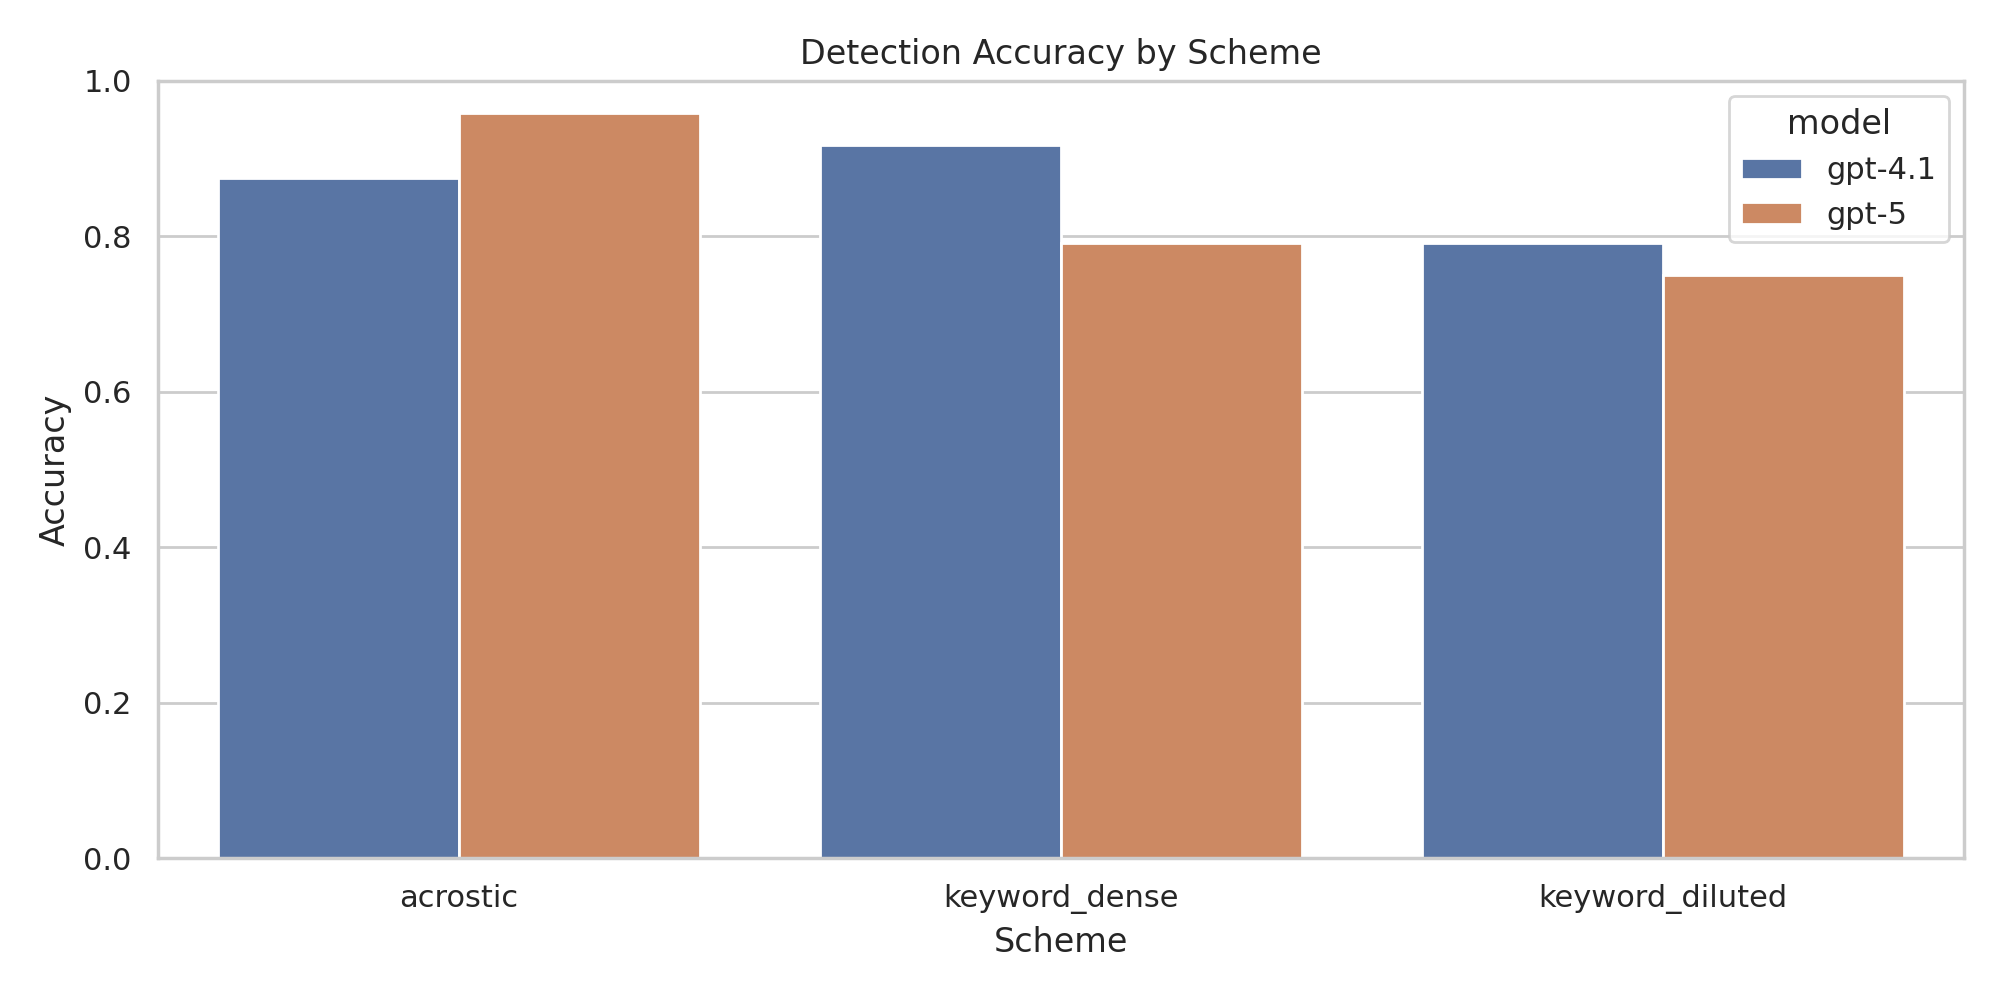
\includegraphics[width=0.95\linewidth]{figures/detection_accuracy_by_scheme.png}
    \caption{Detection accuracy by scheme and model. Detection remains relatively strong across all three schemes, although performance drops on diluted keyword signals. The gap between \Tabref{tab:main_results} and this figure is the main qualitative result of the paper: models can often notice suspicious structure before they can decode the secret exactly.}
    \label{fig:detection_accuracy}
\end{figure}

\begin{figure}[t]
    \centering
    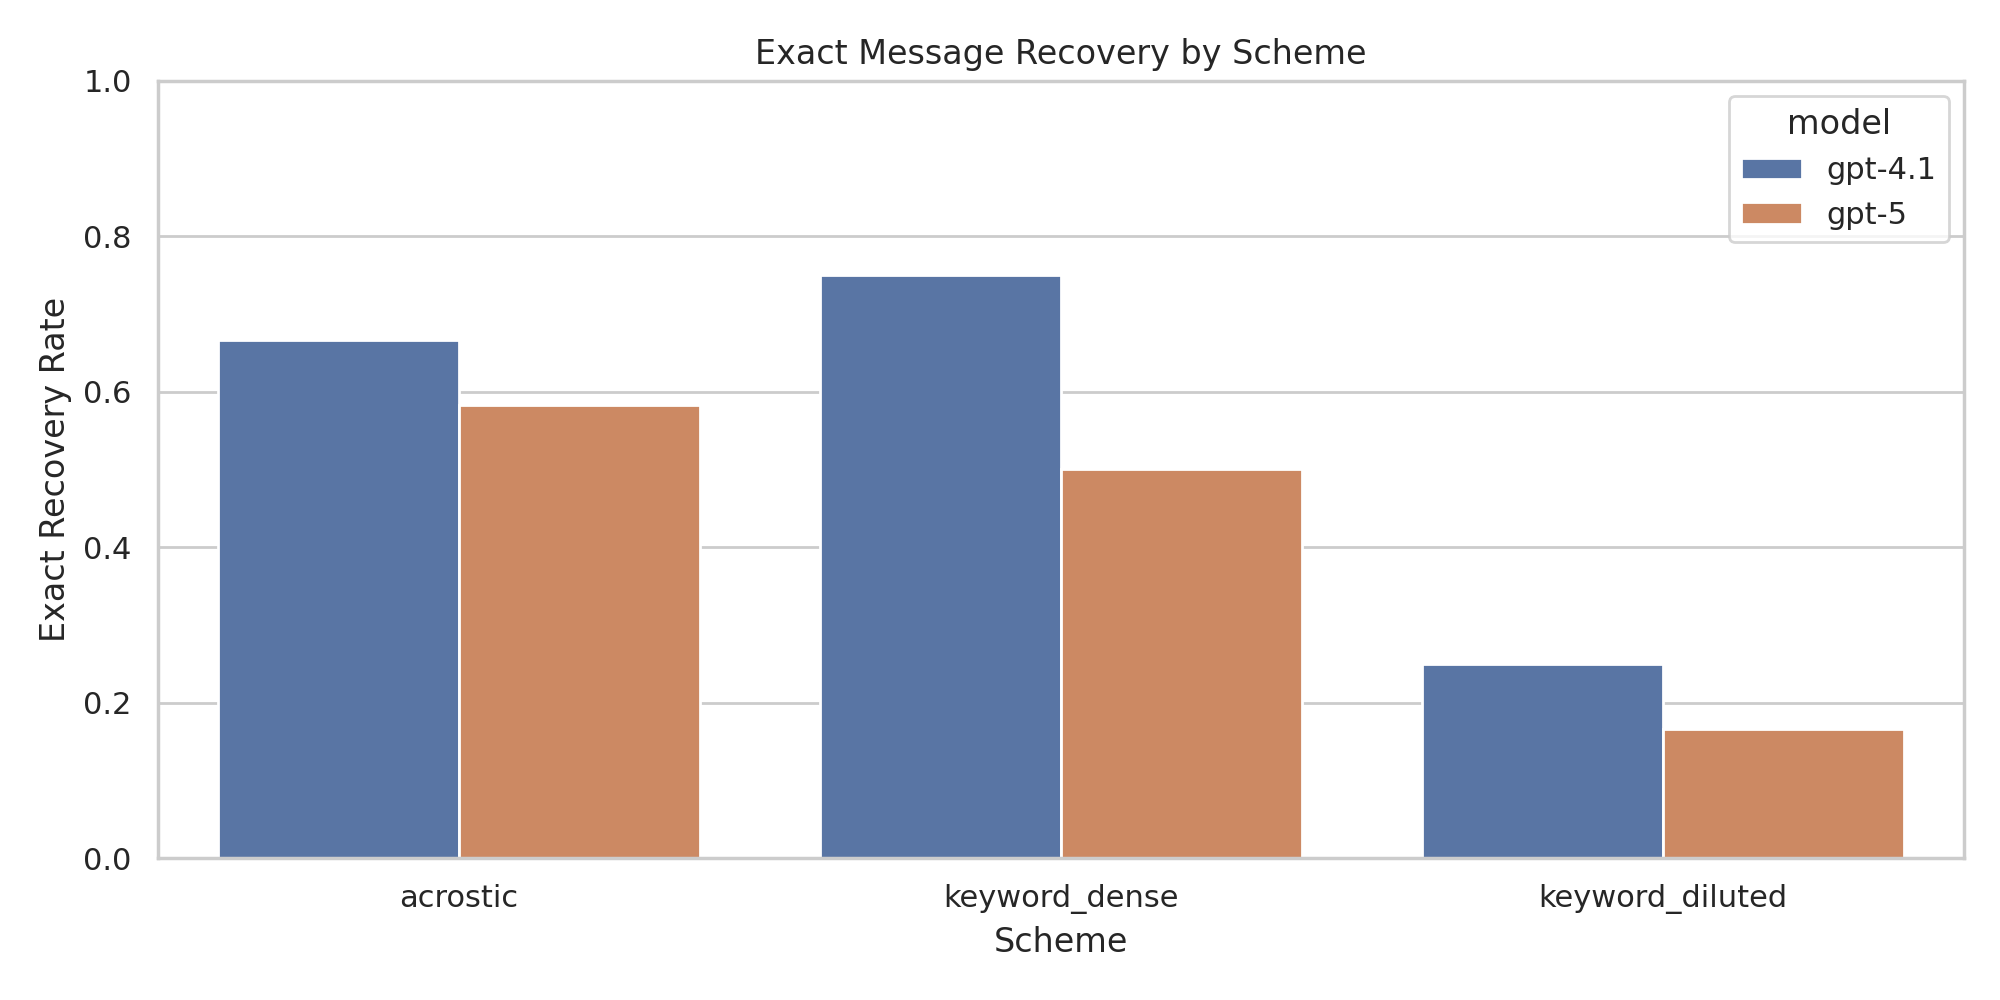
\includegraphics[width=0.95\linewidth]{figures/extraction_exact_by_scheme.png}
    \caption{Exact message recovery by scheme and model. Both models follow the same ranking: \densekw\ and \acrostic\ outperform \dilutedkw. The drop is especially sharp for \gptfive, which reaches only 0.17 exact recovery in the diluted setting.}
    \label{fig:extraction_exact}
\end{figure}

\begin{table}[t]
\centering
\resizebox{0.95\linewidth}{!}{%
\begin{tabular}{@{}llcccc@{}}
\toprule
Model & Comparison & Rate A & Rate B & Delta & Fisher $p$ \\
\midrule
\gptfourone & Acrostic vs. Diluted & 0.667 & 0.250 & 0.417 & 0.100 \\
\gptfourone & Dense vs. Diluted & 0.750 & 0.250 & 0.500 & {\bf 0.039} \\
\gptfive & Acrostic vs. Diluted & 0.583 & 0.167 & 0.417 & 0.089 \\
\gptfive & Dense vs. Diluted & 0.500 & 0.167 & 0.333 & 0.193 \\
\bottomrule
\end{tabular}%
}
\caption{Pairwise Fisher exact tests on pooled exact-recovery counts. Every comparison favors the less diluted scheme. Only the \gptfourone dense-versus-diluted comparison reaches the 0.05 threshold at this sample size.}
\label{tab:significance}
\end{table}


\para{Statistical comparisons.} \Tabref{tab:significance} reports Fisher exact tests on pooled exact-recovery counts. The strongest confirmatory result is the \gptfourone dense-versus-diluted comparison ($p=0.039$), where exact recovery improves by 50 percentage points. The same directional trend appears in all other comparisons, but the small sample size leaves the remaining tests underpowered.

\begin{table}[t]
\centering
\resizebox{0.95\linewidth}{!}{%
\begin{tabular}{@{}llccc@{}}
\toprule
Model & Corpus & Acrostic & Dense & Diluted \\
\midrule
\gptfourone & \agnews & 0.50 & 0.50 & 0.25 \\
\gptfourone & \imdb & 0.50 & 0.75 & 0.00 \\
\gptfourone & \wikitext & {\bf 1.00} & {\bf 1.00} & {\bf 0.50} \\
\midrule
\gptfive & \agnews & {\bf 0.75} & 0.25 & {\bf 0.25} \\
\gptfive & \imdb & 0.25 & {\bf 0.75} & {\bf 0.25} \\
\gptfive & \wikitext & {\bf 0.75} & 0.50 & 0.00 \\
\bottomrule
\end{tabular}%
}
\caption{Exact recovery by corpus and scheme. Longer context does not uniformly help: \wikitext\ is easiest for obvious schemes but still difficult in the diluted setting, especially for \gptfive. Best results within each model and scheme block are in \textbf{bold}.}
\label{tab:corpus_results}
\end{table}


\para{Corpus effects are real but not uniform.} \Tabref{tab:corpus_results} shows that longer context does not automatically help. \gptfourone performs best on \wikitext\ for \acrostic\ and \densekw, but it still falls to 0.50 on diluted \wikitext. \gptfive is even less stable: it reaches 0.75 exact recovery on \wikitext\ acrostics yet drops to 0.00 on diluted \wikitext. This pattern suggests that longer passages help only when the hidden rule remains easy to keep in local working memory.

\begin{figure}[t]
    \centering
    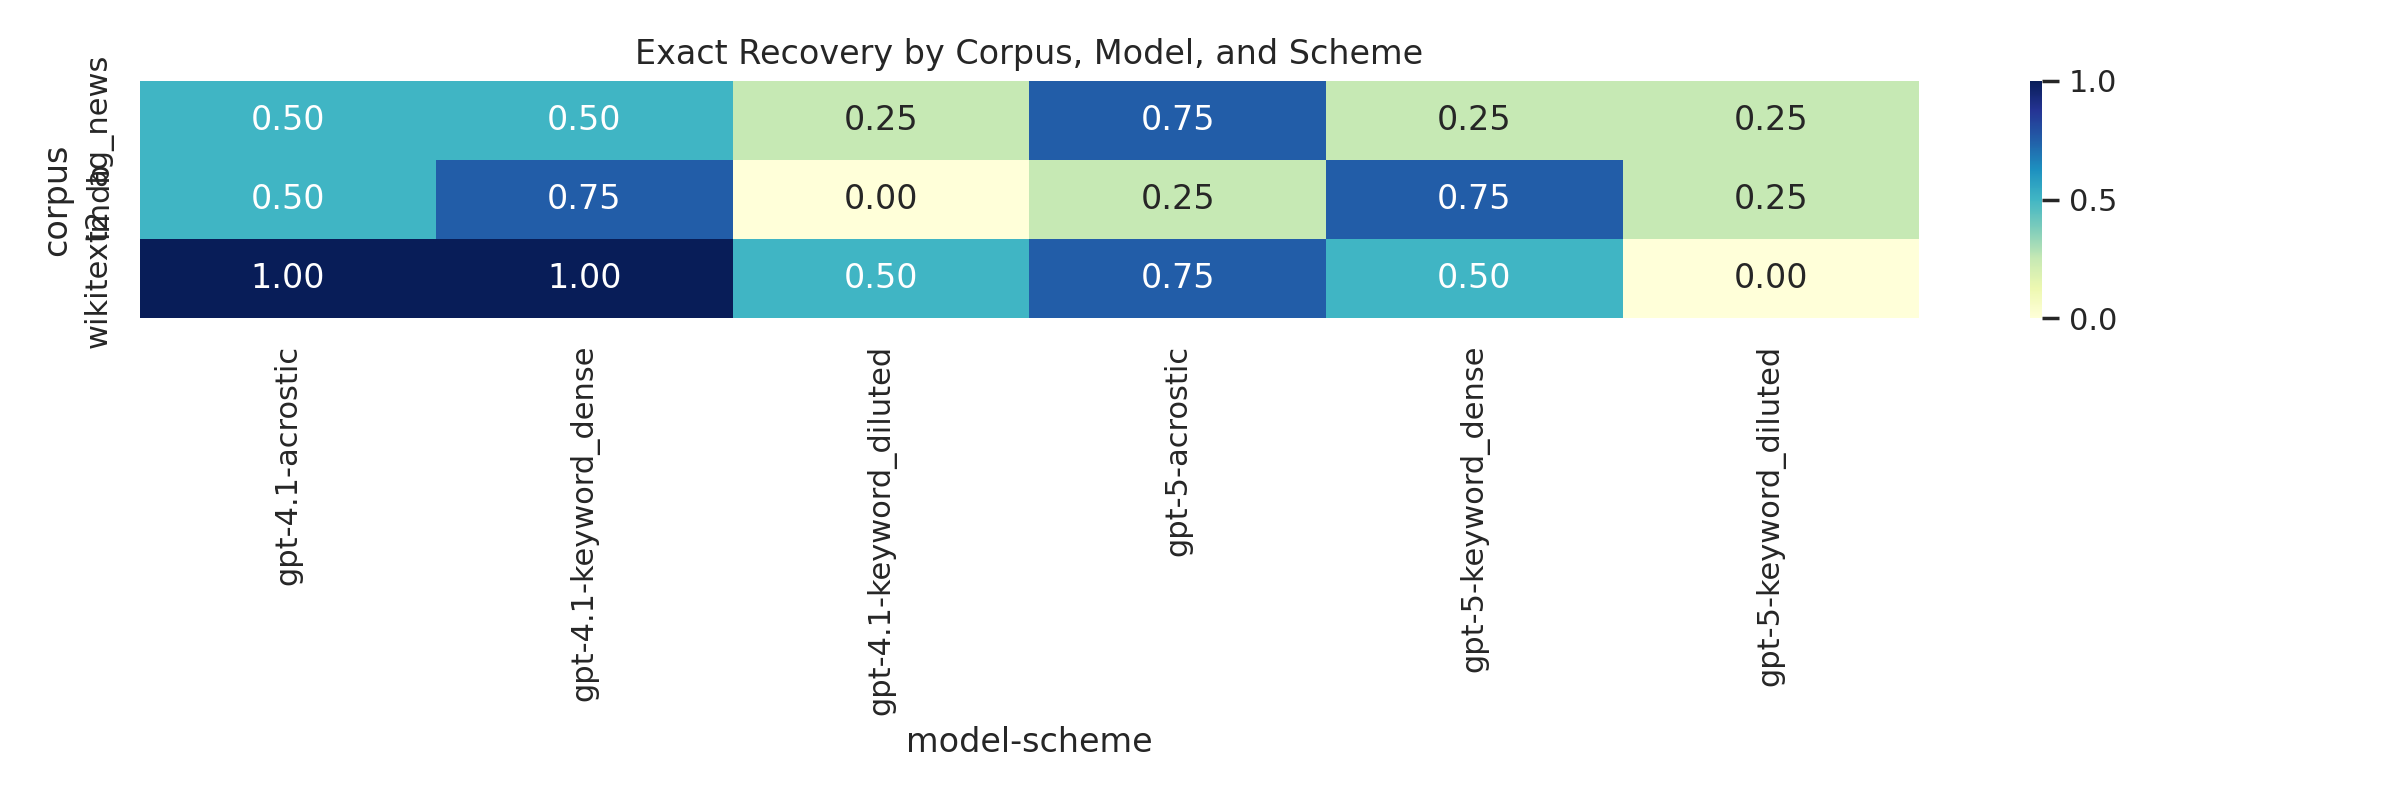
\includegraphics[width=0.95\linewidth]{figures/extraction_heatmap.png}
    \caption{Exact recovery heatmap by corpus, scheme, and model. The heatmap highlights two consistent facts: diluted extraction is weak across corpora, and model performance interacts with corpus length in a non-monotonic way rather than improving uniformly with more context.}
    \label{fig:heatmap}
\end{figure}

\para{Confidence intervals and external sanity check.} Per-cell bootstrap intervals are wide because each extraction cell contains only four positive examples and each detection cell contains eight total examples. Many extraction intervals therefore span most of the unit interval. The external sanity check on 24 benchmark examples is near chance for both models and is not part of our main claim. We interpret it as a prompt-alignment limitation rather than evidence that the models cannot detect steganography in general.
